%   DOCUMENT CLASS  %%%%%%%%%%%%%%%%%%%%%%%%%%%%%%%%%%%%%%%%%%%%%%%%%%%%%%%%%%%
%
%   Use the `sfuthesis` class to format your thesis. If your program does not
%   require a thesis defence, use the class option `undefended` like so:
%
%     \documentclass[undefended]{sfuthesis}
%
%   To generate a signature page for your defence, use the `sfuapproval` class
%   instead, by replacing the below line with
%
%     \documentclass{sfuapproval}
%
%   For more information about thesis formatting requirements, go to
%
%     http://www.lib.sfu.ca/help/publish/thesis
%
%   or ask a thesis advisor at the SFU Research Commons.
%

\documentclass{sfuthesis}



%   DOCUMENT METADATA  %%%%%%%%%%%%%%%%%%%%%%%%%%%%%%%%%%%%%%%%%%%%%%%%%%%%%%%%
%
%   Fill in the following information for the title page and approval page.
%

\title{Learning State-Action Value Functions for Volleyball Data}
\thesistype{Thesis}
\author{Martin Ambrozic}
\previousdegrees{%
	M.Sc., Delft Technical University, 2013\\
	B.Sc., University of Ljubljana, 2011}
\degree{Master of Science}
\discipline{Computing Science}
\department{Department of Computing Science}
\faculty{Faculty of Applied Science}
\copyrightyear{2020}
\semester{Fall 2020}
\date{December 20, 2020}

\keywords{}

\committee{%
	\chair{Chair}{Professor}
	\member{Oliver Schulte}{Senior Supervisor\\Professor}
	\member{Mo Chen}{Internal Examiner\\Assistant Professor\\School of Computing Science}
	\member{Steven Ruuth}{External Examiner\\Professor\\Department of Mathematics}
}



%   PACKAGES %%%%%%%%%%%%%%%%%%%%%%%%%%%%%%%%%%%%%%%%%%%%%%%%%%%%%%%%%%%%%%%%%%
%
%   Add any packages you need for your thesis here.
%   You don't need to call the following packages, which are already called in
%   the sfuthesis class file:
%
%   - appendix
%   - etoolbox
%   - fontenc
%   - geometry
%   - lmodern
%   - nowidow
%   - setspace
%   - tocloft
%
%   If you call one of the above packages (or one of their dependencies) with
%   options, you may get a "Option clash" LaTeX error. If you get this error,
%   you can fix it by removing your copy of \usepackage and passing the options
%   you need by adding
%
%       \PassOptionsToPackage{<options>}{<package>}
%
%   before \documentclass{sfuthesis}.
%
%   The following packages are a few suggestions you might find useful.
%
%   (1) amsmath and amssymb are essential if you have math in your thesis;
%       they provide useful commands like ``blackboard bold'' symbols and
%       environments for aligning equations.
%   (2) amsthm includes allows you to easily change the style and numbering of
%       theorems. It also provides an environment for proofs.
%   (3) graphicx allows you to add images with \includegraphics{filename}.
%   (4) hyperref turns your citations and cross-references into clickable
%       links, and adds metadata to the compiled PDF.
%   (5) pdfpages lets you import pages of external PDFs using the command
%       \includepdf{filename}. You will need to do this if your research
%       requires an Ethics Statement.
%

\usepackage{amsmath}                            % (1)
\usepackage{amssymb}                            % (1)
\usepackage{amsthm}                             % (2)
\usepackage{graphicx}                           % (3)
\usepackage{multirow}
\usepackage{makecell}
\usepackage[pdfborder={0 0 0}]{hyperref}        % (4)
% \usepackage{pdfpages}                         % (5)
% ...
% ...
% ...
% ... add your own packages here!




%   OTHER CUSTOMIZATIONS %%%%%%%%%%%%%%%%%%%%%%%%%%%%%%%%%%%%%%%%%%%%%%%%%%%%%%
%
%   Add any packages you need for your thesis here. We've started you off with
%   a few suggestions.
%
%   (1) Use a single word space between sentences. If you disable this, you
%       will have to manually control spacing around abbreviations.
%   (2) Correct the capitalization of "Chapter" and "Section" if you use the
%       \autoref macro from the `hyperref` package.
%   (3) The LaTeX thesis template defaults to one-and-a-half line spacing. If
%       your supervisor prefers double-spacing, you can redefine the
%       \defaultspacing command.
%

\frenchspacing                                    % (1)
\renewcommand*{\chapterautorefname}{Chapter}      % (2)
\renewcommand*{\sectionautorefname}{Section}      % (2)
\renewcommand*{\subsectionautorefname}{Section}   % (2)
% \renewcommand{\defaultspacing}{\doublespacing}  % (3)
% ...
% ...
% ...
% ... add your own customizations here!




%   FRONTMATTER  %%%%%%%%%%%%%%%%%%%%%%%%%%%%%%%%%%%%%%%%%%%%%%%%%%%%%%%%%%%%%%
%
%   Title page, committee page, copyright declaration, abstract,
%   dedication, acknowledgements, table of contents, etc.
%
%   If your research requires an Ethics Statement, download one from the
%   SFU library website and uncomment the appropriate lines below.
%

\begin{document}
	
	\frontmatter
	\maketitle{}
	\makecommittee{}
	
	\begin{abstract}
		This is a blank document from which you can start writing your thesis.
	\end{abstract}
	
	
	\begin{dedication}
		This is an optional page.
	\end{dedication}
	
	
	\begin{acknowledgements}
		This is an optional page.
	\end{acknowledgements}
	
	\addtoToC{Table of Contents}%
	\tableofcontents%
	\clearpage
	
	\addtoToC{List of Tables}%
	\listoftables%
	\clearpage
	
	\addtoToC{List of Figures}%
	\listoffigures%
	\clearpage
	
	
	
	
	
	%   MAIN MATTER  %%%%%%%%%%%%%%%%%%%%%%%%%%%%%%%%%%%%%%%%%%%%%%%%%%%%%%%%%%%%%%
	%
	%   Start writing your thesis --- or start \include ing chapters --- here.
	%
	
	\mainmatter%
	
	%\chapter{Introduction}
	
	%By default, only works cited in the text will be added to the bibliography~\cite{latexcompanion}.
	
	\chapter{Dataset and Modelling}
	
	\section{Dataset Description}
	The volleyball dataset was collected in collaboration with the University of British Columbia's men's volleyball programme. The UBC Thunderbirds compete in the Canada West division of U-Sports volleyball, which is the highest level of volleyball university competition in Canada. Their regular season consists of a double round robin phase, where they play each of the other Canada West teams twice, and a play-off phase, where top seeded teams play a single elimination bracket to determine the conference champion as well as participants in the U-Sports national final tournament. During the data collection time window, 12 teams participated in the Canada West competition, except in 2017/2018, where 13 teams competed.\\\\
	The collection process was manual, using specialized software to record play-by-play data, either live at the game or after the fact using game video. In the former case, a second pass was needed to ensure quality and completeness of data. The format used was introduced by the company Data Project based in Salerno, Italy and has become widely adopted in professional and international volleyball. Both teams' actions were included for every game.\\\\
	The dataset contains data from all games played by UBC over three seasons. Additionally, some matches between other teams in Canada West were included, originally intended for the purpose of tactical preparation for an upcoming opponent. In numbers, the data contains:
	\begin{itemize}
		\item 204 games,
		\item 764 sets,
		\item 34,242 rallies,
		\item 146,050 game events.
	\end{itemize}
	Each entry in the dataset corresponds to an action event by a player in the game. We differentiate 7 action types:
	\begin{itemize}
		\item \textbf{Serve}: first contact of the serving team, the action of putting the ball into play over the net from behind the baseline.
		\item \textbf{Receive}: first contact of the team receiving the opponent's serve.
		\item \textbf{Set}: Second contact on either side, the aim of which is to deliver the ball to an attacker.
		\item \textbf{Attack}: Usually the third contact of either team, spiking the ball over the net with the aim of scoring by hitting the ground in the opponent's court.
		\item \textbf{Block}: The action of one or more players by the net attempting to defending against an attack by deflecting the ball back to the opponent's court as it crosses the net.
		\item \textbf{Dig}: The defensive action against an opponent's attack, volleying the ball before it contacts the ground.
		\item \textbf{Free-ball}: The first contact of a team after the opposing team failed to produce a proper attack and volleyed an 'easy ball' over the net.
	\end{itemize}
	Further, the outcome of each action is recorded, ranging from '=' (double negative), through '-' (negative), '/', '!', '+' (positive) and '\#' (double positive). The meanings of these symbols vary by action type, but in general double negative corresponds to an error (awarding the rally to the opponent) and double positive is a winning or perfect outcome, eg. a scoring attack.\\\\
	For most actions, the execution location is also recorded, as well as the trajectory location for attack and serve actions. Finally, we also record the context, i.e. the state of the game, including the current set number (1 through maximum 5) and the points scored by each team in the current set (usually between 0 and 25, but can be higher in a 'win by 2' scenario). Table \ref{tab:data-fields} summarizes the context and action-related fields recorded in the dataset.
	\begin{table}[ht]
		\centering
		\begin{tabular}{c|c|c|c|c}
			\textbf{Action Field} & \textbf{Player, Team} & \textbf{Type} & \textbf{Outcome} & \textbf{Location, Trajectory}         \\ \hline
			\textbf{Range} & categorical           & 7 categories  & 6 categories     & \makecell[c]{Discretized\\ 12-by-6 grid of locations}
		\end{tabular}
		\\ \vspace{0.75cm}
		\begin{tabular}{c|c|c}
			\textbf{Context Field} & \textbf{Set Number} & \textbf{Set Scores}    \\ \hline
			\textbf{Range} & Integers 1-5        & Integers 0-31 per team
		\end{tabular}
		\caption{Summary of fields in the volleyball dataset. Action-related fields on top, context-related fields on the bottom.}
		\label{tab:data-fields}
	\end{table}
	
	\chapter{Model Evaluation}
	
	\section{Comparing Action Values Between Models}
	
	We compare action values computed by the different models for the home and away team, including all possible action types and outcomes. Tables \ref{tab:qvalues_home} and \ref{tab:qvalues_away} contain mean values of $Q(s,a)$ over all state-action pairs where the action type and outcome for $a$ are fixed, separately for the home team and away team, respectively.\\\\
	Note that there is no inherent order in the outcome symbols and the values for the different outcomes are entirely learned by the models. The fact that action values increase for outcomes generally considered more favourable is a good sanity check and provides validation for our models. We also compute mean eventual rewards directly from the data for comparison. Overall the model values seem to agree well with the data averages with a few exceptions. For example, home values for serve outcomes '+' and '!' computed by the decision tree model are identical and seem to be somewhere in between the correct values, suggesting that a split failed to occur and samples were grouped together in the same leaf node. The same can be observed for the '!' and '+' outcomes of the away receive action. The random forest model corrects this to some extent, but still outputs a positive value for the '!' outcome, contrary to what the data suggests.
	
	\begin{table}
		\centering
		\begin{tabular}{ccccccc}
			\multicolumn{7}{c}{\textbf{Home Action Values}} \\
			\textbf{Skill} & \multicolumn{1}{c|}{\textbf{Outcome}} & \textbf{Dec. Tree} & \textbf{Rand. Forest} & \textbf{Neural Net.} & \multicolumn{1}{c|}{\textbf{Mimic Tree}} & \textbf{Data} \\ \hline
			S              & \multicolumn{1}{c|}{=}                & -1                 & -1                    & -0.998               & \multicolumn{1}{c|}{-0.998}              & -1            \\
			& \multicolumn{1}{c|}{-}                & -0.293             & -0.291                & -0.29                & \multicolumn{1}{c|}{-0.29}               & -0.293        \\
			& \multicolumn{1}{c|}{!}                & 0.103              & 0.011                 & -0.101               & \multicolumn{1}{c|}{-0.101}              & -0.106        \\
			& \multicolumn{1}{c|}{+}                & 0.103              & 0.246                 & 0.225                & \multicolumn{1}{c|}{0.225}               & 0.238         \\
			& \multicolumn{1}{c|}{\#}               & 1                  & 1                     & 0.997                & \multicolumn{1}{c|}{0.998}               & 1             \\ \hline
			R              & \multicolumn{1}{c|}{=}                & -1                 & -1                    & -0.998               & \multicolumn{1}{c|}{-0.998}              & -1            \\
			& \multicolumn{1}{c|}{-}                & -0.167             & -0.167                & -0.157               & \multicolumn{1}{c|}{-0.157}              & -0.166        \\
			& \multicolumn{1}{c|}{!}                & 0.104              & 0.039                 & 0.11                 & \multicolumn{1}{c|}{0.108}               & 0.118         \\
			& \multicolumn{1}{c|}{+}                & 0.287              & 0.323                 & 0.325                & \multicolumn{1}{c|}{0.325}               & 0.321         \\
			& \multicolumn{1}{c|}{\#}               & 0.437              & 0.427                 & 0.446                & \multicolumn{1}{c|}{0.446}               & 0.446         \\ \hline
			A              & \multicolumn{1}{c|}{=}                & -0.991             & -0.987                & -0.994               & \multicolumn{1}{c|}{-0.993}              & -1            \\
			& \multicolumn{1}{c|}{/}                & -0.984             & -0.968                & -0.993               & \multicolumn{1}{c|}{-0.986}              & -1            \\
			& \multicolumn{1}{c|}{-}                & 0.02               & -0.052                & -0.072               & \multicolumn{1}{c|}{-0.072}              & -0.071        \\
			& \multicolumn{1}{c|}{!}                & 0.107              & 0.082                 & 0.122                & \multicolumn{1}{c|}{0.117}               & 0.127         \\
			& \multicolumn{1}{c|}{+}                & 0.302              & 0.284                 & 0.372                & \multicolumn{1}{c|}{0.368}               & 0.362         \\
			& \multicolumn{1}{c|}{\#}               & 0.947              & 0.99                  & 0.994                & \multicolumn{1}{c|}{0.994}               & 1             \\ \hline
			B              & \multicolumn{1}{c|}{=}                & -0.87              & -0.969                & -0.99                & \multicolumn{1}{c|}{-0.961}              & -1            \\
			& \multicolumn{1}{c|}{-}                & -1                 & -1                    & -0.993               & \multicolumn{1}{c|}{-0.993}              & -1            \\
			& \multicolumn{1}{c|}{!}                & 0.103              & 0.209                 & 0.063                & \multicolumn{1}{c|}{0.071}               & 0.052         \\
			& \multicolumn{1}{c|}{+}                & 0.218              & 0.154                 & 0.146                & \multicolumn{1}{c|}{0.145}               & 0.142         \\
			& \multicolumn{1}{c|}{\#}               & 0.999              & 1                     & 0.993                & \multicolumn{1}{c|}{0.993}               & 1             \\ \hline
			D              & \multicolumn{1}{c|}{=}                & -1                 & -1                    & -0.995               & \multicolumn{1}{c|}{-0.995}              & -1            \\
			& \multicolumn{1}{c|}{!}                & -0.289             & -0.262                & -0.278               & \multicolumn{1}{c|}{-0.275}              & -0.282        \\
			& \multicolumn{1}{c|}{\#}               & 0.217              & 0.152                 & 0.155                & \multicolumn{1}{c|}{0.155}               & 0.147         \\ \hline
			E              & \multicolumn{1}{c|}{=}                & -0.941             & -0.986                & -0.994               & \multicolumn{1}{c|}{-0.989}              & -1            \\
			& \multicolumn{1}{c|}{+}                & 0.364              & 0.375                 & 0.371                & \multicolumn{1}{c|}{0.371}               & 0.372        
		\end{tabular}
		\caption{Comparison of action values computed by different models. Values shown are mean state-action values $Q(s,a)$, where the action type (skill) and outcome are specified in the table. Negative values correspond to the away team having a higher probability of winning the rally. Additionally, the Data column contains expected rewards computed directly from the dataset samples.}
		\label{tab:qvalues_home}
	\end{table}
	
	\begin{table}
		\centering
		\begin{tabular}{ccccccc}
			\multicolumn{7}{c}{\textbf{Away Action Values}}                                                                                                                                       \\
			\textbf{Skill} & \multicolumn{1}{c|}{\textbf{Outcome}} & \textbf{Dec. Tree} & \textbf{Rand. Forest} & \textbf{Neural Net.} & \multicolumn{1}{c|}{\textbf{Mimic Tree}} & \textbf{Data} \\ \hline
			S              & \multicolumn{1}{c|}{=}                & 1                  & 1                     & 0.999                & \multicolumn{1}{c|}{0.999}               & 1             \\
			& \multicolumn{1}{c|}{-}                & 0.362              & 0.351                 & 0.364                & \multicolumn{1}{c|}{0.364}               & 0.362         \\
			& \multicolumn{1}{c|}{!}                & 0.107              & 0.11                  & 0.11                 & \multicolumn{1}{c|}{0.11}                & 0.118         \\
			& \multicolumn{1}{c|}{+}                & -0.166             & -0.167                & -0.157               & \multicolumn{1}{c|}{-0.158}              & -0.167        \\
			& \multicolumn{1}{c|}{\#}               & -1                 & -1                    & -0.998               & \multicolumn{1}{c|}{-0.997}              & -1            \\ \hline
			R              & \multicolumn{1}{c|}{=}                & 1                  & 1                     & 0.998                & \multicolumn{1}{c|}{0.998}               & 1             \\
			& \multicolumn{1}{c|}{-}                & 0.239              & 0.239                 & 0.225                & \multicolumn{1}{c|}{0.225}               & 0.238         \\
			& \multicolumn{1}{c|}{!}                & -0.185             & -0.097                & -0.101               & \multicolumn{1}{c|}{-0.1}                & -0.106        \\
			& \multicolumn{1}{c|}{+}                & -0.185             & -0.251                & -0.252               & \multicolumn{1}{c|}{-0.252}              & -0.256        \\
			& \multicolumn{1}{c|}{\#}               & -0.369             & -0.368                & -0.373               & \multicolumn{1}{c|}{-0.373}              & -0.369        \\ \hline
			A              & \multicolumn{1}{c|}{=}                & 0.986              & 0.987                 & 0.994                & \multicolumn{1}{c|}{0.986}               & 1             \\
			& \multicolumn{1}{c|}{/}                & 0.927              & 0.965                 & 0.993                & \multicolumn{1}{c|}{0.99}                & 1             \\
			& \multicolumn{1}{c|}{-}                & 0.114              & 0.151                 & 0.155                & \multicolumn{1}{c|}{0.156}               & 0.153         \\
			& \multicolumn{1}{c|}{!}                & 0.091              & 0.103                 & 0.067                & \multicolumn{1}{c|}{0.072}               & 0.051         \\
			& \multicolumn{1}{c|}{+}                & -0.204             & -0.206                & -0.287               & \multicolumn{1}{c|}{-0.275}              & -0.277        \\
			& \multicolumn{1}{c|}{\#}               & -0.998             & -0.992                & -0.994               & \multicolumn{1}{c|}{-0.993}              & -1            \\ \hline
			B              & \multicolumn{1}{c|}{=}                & 0.951              & 0.969                 & 0.992                & \multicolumn{1}{c|}{0.991}               & 1             \\
			& \multicolumn{1}{c|}{-}                & 0.999              & 1                     & 0.994                & \multicolumn{1}{c|}{0.994}               & 1             \\
			& \multicolumn{1}{c|}{!}                & 0.116              & 0.109                 & 0.123                & \multicolumn{1}{c|}{0.119}               & 0.127         \\
			& \multicolumn{1}{c|}{+}                & -0.052             & -0.07                 & -0.072               & \multicolumn{1}{c|}{-0.071}              &               \\
			& \multicolumn{1}{c|}{\#}               & -1                 & -0.999                & -0.993               & \multicolumn{1}{c|}{-0.993}              & -1            \\ \hline
			D              & \multicolumn{1}{c|}{=}                & 1                  & 1                     & 0.995                & \multicolumn{1}{c|}{0.995}               & 1             \\
			& \multicolumn{1}{c|}{!}                & 0.37               & 0.363                 & 0.377                & \multicolumn{1}{c|}{0.378}               & 0.371         \\
			& \multicolumn{1}{c|}{\#}               & -0.069             & -0.071                & -0.064               & \multicolumn{1}{c|}{-0.064}              & -0.062        \\ \hline
			E              & \multicolumn{1}{c|}{=}                & 0.971              & 0.987                 & 0.993                & \multicolumn{1}{c|}{0.989}               & 1             \\
			& \multicolumn{1}{c|}{+}                & -0.281             & -0.287                & -0.283               & \multicolumn{1}{c|}{-0.284}              & -0.281       
		\end{tabular}
		\caption{Comparison of away action values computed by different models. See Table \ref{tab:qvalues_home}}.
		\label{tab:qvalues_away}
	\end{table}
	
	\section{Rally Win Prediction Accuracy}
	The state-action value function has a range of $[-1,1]$ where positive values correspond to higher expected reward for the home team and negative values correspond to higher expected reward for the away team. Denoting by $(s,a)$ the current state-action pair, Q function values can be converted to rally-winning probabilities by using the formula:
	\begin{equation}
		P_H(s,a) = \frac{Q(s,a)+1}{2}
		\label{eq:q_to_prob}
	\end{equation}
	for the home team and
	\begin{equation}
		P_A(s,a) = \frac{1-Q(s,a)}{2}
	\end{equation}
	for the away team. These probabilities can be used to predict the eventual winner of the rally and evaluate accuracy differences between our models. Table \ref{tab:class_accuracy} shows prediction accuracies as well as cross entropy values over the entire dataset for the different models. Cross entropy for a single prediction is computed using the formula
	\begin{equation}
		-\log P(y|P_H) = - (y \log P_H + (1-y) \log(1-P_H)),
	\end{equation}
	where $y \in \{0,1\}$ is the indicator variable for the home team eventually winning the current rally and $P_H$ is the according predicted home win probability. Dependency of $y$ and $P_H$ on $s$ and $a$ omitted here for brevity.\\\\
	We consider some baselines in this context, against which to compare model accuracy. The home team has a slight advantage, so always predicting home is a possible baseline. Furthermore, the receiving team normally scores more often than the serving team, so always predicting the receiving team is another viable baseline. We find the following baseline accuracies are obtained:
	\begin{itemize}
		\item Always predicting home team wins the rally: 0.5174,
		\item Always predicting receiving team wins the rally: 0.5807.
	\end{itemize}
	From Table \ref{tab:class_accuracy} accuracy values, clearly all models perform well above the considered baselines, but the random forest model outperforms the rest with a prediction accuracy of just over 80\%, which suggests it as the best choice in the win prediction context. Despite the prediction accuracy advantage however, we will find that random forest is not the best choice when it comes to preserving state-action value properties inherited from the Markov decision process.\\
	\begin{table}
		\centering
		\begin{tabular}{c|cc}
			\textbf{Model} & \textbf{Accuracy Score} & \textbf{Log Loss} \\ \hline
			Decision Tree  & 0.7493                  & 0.4345            \\
			Random Forest  & 0.8092                  & 0.4017            \\
			Neural Network & 0.7551                  & 0.4283            \\
			Mimic Tree     & 0.7529                  & 0.4301           
		\end{tabular}
		\caption{Comparison of models for rally win prediction.}
		\label{tab:class_accuracy}
	\end{table}
	\\To further analyse the win prediction capabilities of our models, we consider predictions depending on how many actions remain in the rally. Recall that the model input is a partial sequence of actions leading up to the current state and action, which means model performance likely depends significantly on how much play remains in the current rally. Figure \ref{fig:acc-vs-dist} shows a graph of this dependency. When the observed action is the last one in the rally (i.e. zero actions remain), win prediction accuracy is perfect for all considered models. It remains significantly better than guessing for up to 4 actions away from the rally terminating, but for distances of 5 or higher, accuracy is significantly impaired and only the random forest model continues to give predictions with around 60\% accuracy.
	\begin{figure}
		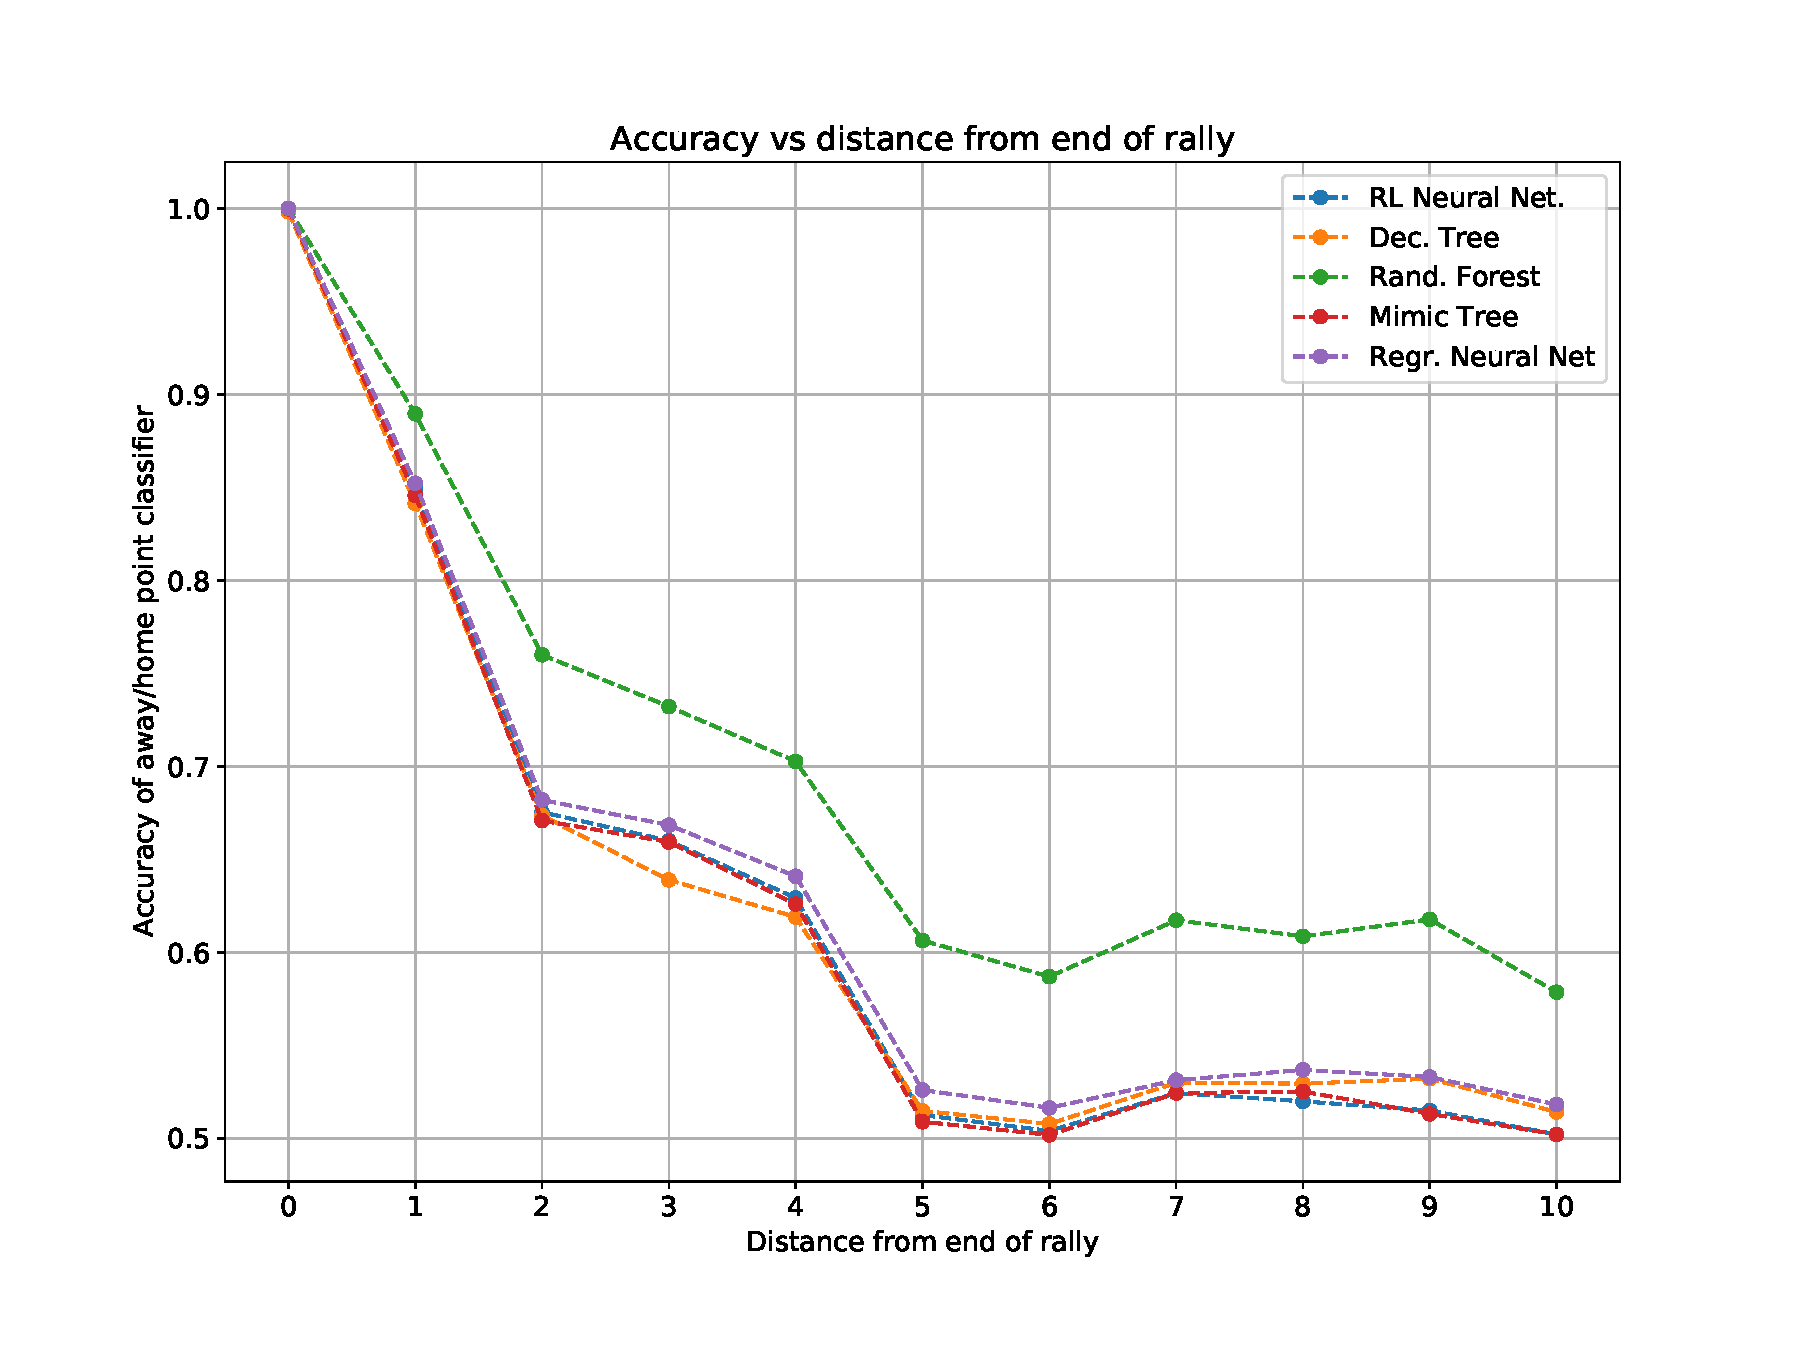
\includegraphics[scale=0.55]{img/acc_vs_dist.pdf}
		\caption{Model win prediction accuracy plotted against distance from the end of rally in terms of actions remaining.}
		\label{fig:acc-vs-dist}
	\end{figure}
	
	\section{Temporal Consistency}
	
	The action-value function $Q_\pi$ for a given policy $\pi$ over a Markov decision process satisfies a recursive relationship in terms of the current state-action pair $(s,a)$ and possible future state-action pairs $(S_{t+1},A_{t+1})$: 
	\begin{align}
		Q_\pi(s,a) &= \mathbb{E} \left[  R_{t+1} + \gamma Q_{\pi}(S_{t+1}, A_{t+1}) \, | \, S_t = s, A_t = a \right]\\
		&=  R_{t+1} + \sum_{s' \in S, a' \in A} \gamma P(S_{t+1} = s', A_{t+1} = a' | S_t = s, A_t = a) Q_\pi(s',a').
	\end{align}
	This property is known as the Bellman equation \cite{sutton2018reinforcement} and it gives us the opportunity to verify the quality of our action-value estimates in an aspect that is different from what we did so far. If our approximation is indeed an action-value function, we expect it to (at least approximately) agree with the Bellman equation in addition to minimizing the loss function against the training data.\\\\
	In our context we use a discount factor of $\gamma = 1$ and rewards only occur at episode-ending states. If $s$ is not a terminal state, $R_{t+1} = 0$ and the Bellman equation becomes
	\begin{equation}
		Q(s,a) = \sum_{s',a'} P(S_{t+1} = s', A_{t+1} = a' | S_t = s, A_t = a) Q(s',a').
		\label{eq:markov_diff}
	\end{equation}
	Assuming we've computed an action-value function estimate for all the states in our dataset, we can proceed to verify this equality using the data, since the transition probability $P$ can be estimated by counting occurrences of states in the dataset (denoted by $c$) as
	$$P(S_{t+1} = s', A_{t+1} = a' | S_t = s, A_t = a) = \frac{c(S_{t+1} = s', A_{t+1} = a', S_t = s, A_t = a)}{c(s,a)}.$$
	Furthermore, since the state space is large, we wish to avoid examining a single state due to potential data sparsity effects. We will instead be interested in a set of state-action pairs $X$, summing all the corresponding state-action values as they appear in the dataset, namely the quantity:
	$$\sum_{s,a\in X} c(s,a)Q(s,a).$$
	Using \eqref{eq:markov_diff}, we obtain the right hand side:
	\begin{equation}
		\sum_{s,a\in X} c(s,a)Q(s,a) = \sum_{s,a\in X} c(s,a)\sum_{s',a'\in S\times A} \frac{c(s',a',s,a)}{c(s,a)} Q(s',a'),
	\end{equation}
	which simplifies to
	\begin{equation}
		\sum_{s,a\in X} c(s,a)Q(s,a) = \sum_{s,a\in X} \sum_{s',a'\in S\times A} c(s',a',s,a) Q(s',a').
		\label{eq:markov_num}
	\end{equation}
	This final form is the one we use to compute the Bellman equation agreement, since both the left and right hand sides can be computed in a simple loop over the dataset sequences. We are interested in how much our action-value estimates violate \eqref{eq:markov_num}, i.e. the quantity
	\begin{equation}
		e_X = |\sum_{s,a\in X} c(s,a)Q(s,a) - \sum_{s,a\in X} \sum_{s',a'\in S\times A} c(s',a',s,a) Q(s',a') |.
		\label{eq:markov_num2}
	\end{equation}
	We choose the state-action subset $X$ to include actions of a single type with only non-terminal outcomes (for example, we include all serve actions that do not result in an immediate error or point won). We compute the quantity $e_X$ for various action types and compare results across different action-value function approximations.\\\\
	Looking at the $e_X$ values shown in Table \ref{tab:bellman-agreement}, the neural network exhibits overall highest agreement with the Bellman equation and the single decision tree is the worst of our models in this respect. Since the neural network is trained using reinforcement learning principles, in particular because the loss function incorporates the temporal difference target 
	$$Q(s,a) \leftarrow Q(s,a) + \alpha (r + \gamma Q(s', a') - Q(s,a)),$$
	where the state-action pair $(s,a)$ is followed by $(s',a')$ in the data, it is not surprising that temporal consistency is best maintained using this model. Decision tree and random forest models are trained under the assumption of independent data and do not incorporate any information about the sequential nature of the volleyball data. Their $e_X$ values are accordingly much larger and in the case of random forest could outweigh its lower mean squared error compared to the neural network. The mimic tree's $e_X$ seems to be close to the neural network's in most cases, but significantly higher for attack and block actions, which puts it somewhere between the neural network and the random forest overall.
	
	\begin{table}
		\centering
		\begin{tabular}{c|cccccc}
			\textbf{Model}    & \textbf{Serve} & \textbf{Receive} & \textbf{Attack} & \textbf{Set} & \textbf{Block} & \textbf{Dig} \\ \hline
			Decision Tree     & 0.0158                  & 0.0151                    & 0.0376                   & 0.0074                & 0.0641                  & 0.0662                \\
			Random Forest     & 0.0172                  & 0.0183                    & 0.0075                   & 0.0066                & 0.0025                  & 0.0148                \\
			RL Neural Network & 0.0001                  & 0.0005                    & 0.0003                   & 0.0019                & 0.0008                  & 0.0002                \\
			Mimic Tree        & 0.0001                  & 0.0001                    & 0.0076                   & 0.0018                & 0.0125                  & 0.0009               
		\end{tabular}
		\caption{Table of Bellman equation agreement error $e_X$ for various sets of non-terminal states $X$. For each volleyball action type (columns), the set $X$ includes actions performed by the home team with a non-terminal outcome.}
		\label{tab:bellman-agreement}
	\end{table}
	
	\chapter{Q Function Use Examples}
	\section{Serve Risk Assessment}
	The serve action is one of the most crucial actions types in volleyball as its outcome has a large impact on the odds of either team winning the rally. It is also the only action in volleyball where the player executing it has complete control independently of other players' actions. Optimizing the risk/reward profile for serving is therefore an important problem coaches and players frequently face \cite{burton2015linear}. In this section we examine serve action value depending on the score context, namely how close to ending the current set is in terms of score. We take $\max(\text{home score}, \text{away score})$ to be the progress measure of the current set and compare the action values of serves resulting in the '-' and '!' outcomes. The '-' outcome corresponds to the opponent team receiving the ball well enough to have all attack options available - this is the expected outcome of a serve executed with low risk. The '!' serve outcome means the opponent reception landed away from the net, removing the quick middle attack option and making opponent offence more predictable - this is generally the outcome sought when executing a serve with some (controlled) risk.\\\\
	Figure \ref{fig:serve-risk} shows action values converted to point scoring probability (see equation \eqref{eq:q_to_prob}) for the serve outcomes above depending on the current set score. For simplicity, the set score is bracketed into intervals of 0-5, 6-10, 11-15, 16-20 and 21-25. The x axis labels correspond to the upper end of each interval. From the graph we can observe a decreasing trend in the '-' outcome value and an increasing trend in the '!' outcome value. This would suggest a strategy using lower risk serving in the beginning of a set and gradually increasing the risk towards the end of the set, since '!' outcomes become more valuable as the set progresses.\\\\
	This is of course not a complete risk assessment, since we did not include any information regarding serve errors, but it can serve as an example of potential use of the action value function.
	
	\begin{figure}
		\centering
		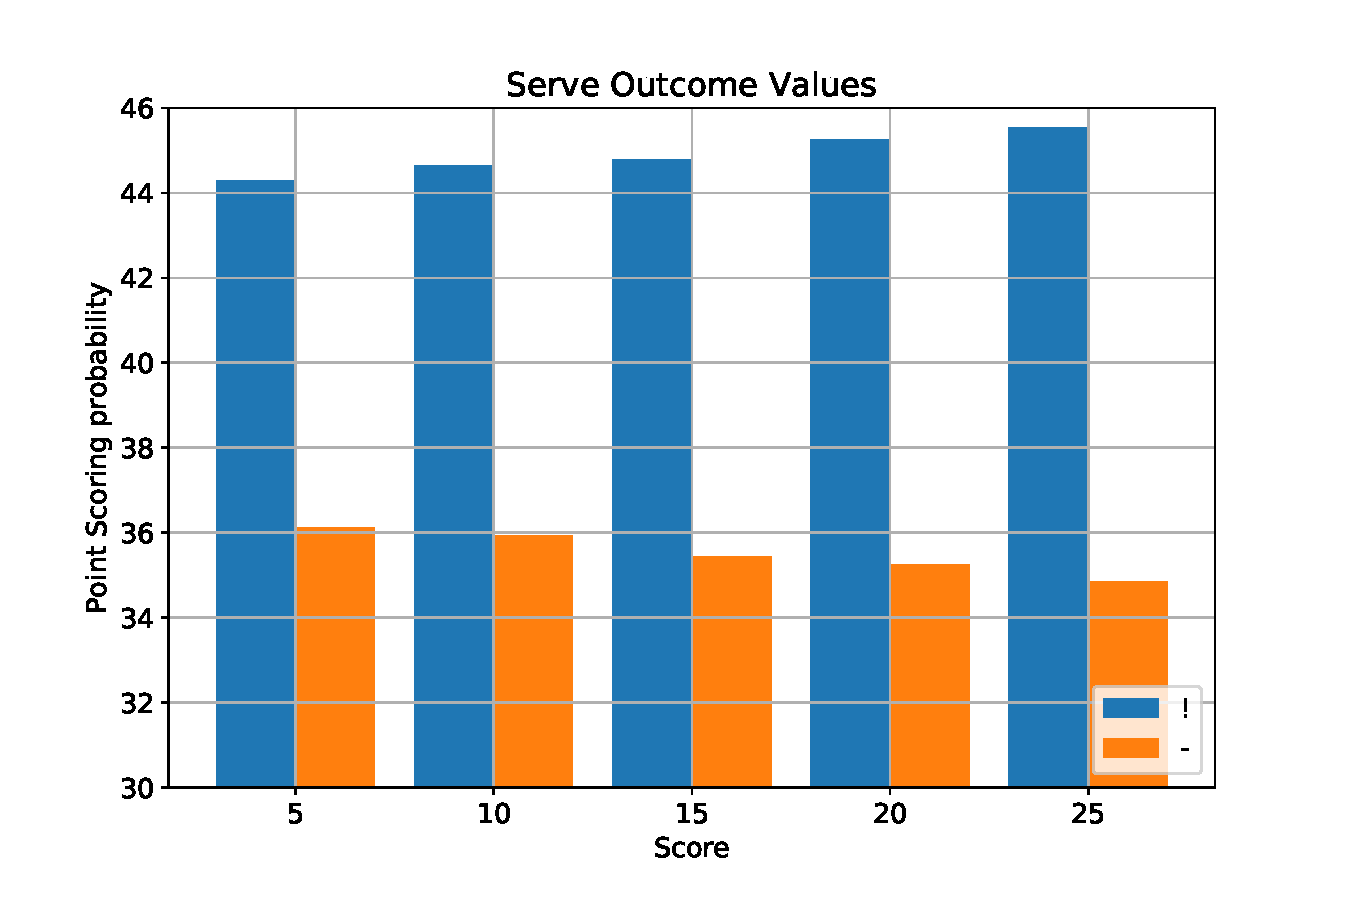
\includegraphics[scale=0.6]{img/serve_risk.pdf}
		\caption{Home serve values converted to point scoring probability for the '-' and '!' serve outcomes depending on current set score.}
		\label{fig:serve-risk}
	\end{figure}
	
	\section{Action Impact}
	
	One of the motivations of computing the action-value function for sports data is the ability to numerically rank teams and players according to their action values. To achieve this, we need to consider that the context of an action performed by a player influences the quality of their actions. Namely, scoring a point from a favorable situation (eg. a successful attack following a perfect pass) should be treated differently than scoring in a situation that is deemed difficult. This leads us to the notion of action impact.\\\\
	As discussed in \cite{routley2015markov}, there are several options of how we could choose to value actions. We will adopt the difference of consecutive action values as a measure of impact. Namely, for a transition from state $s_{t-1}$ to $s_t$, with actions $a_{t-1}$ and $a_t$ we define the impact of $(s_t, a_t)$ as:
	\begin{equation}
		\text{impact}(s_t,a_t) = Q(s_t,a_t) - Q(s_{t-1},a_{t-1}).
		\label{eq:action_impact}
	\end{equation}
	This allows us to capture to some degree how the flow of the game changed when action $a_t$ was performed. This version of valuing player actions was successfully used in the hockey context in \cite{liu2018deep} for player evaluations.\\\\
	Note that since action impact relates to the values of both current and previous states, we need to find a treatment for the first action of any episode (in volleyball this is always a serve action), where $s_{t-1}$ and $a_{t-1}$ are not defined. The most obvious solution is to use an initial state-action value of 0, but since the serving team is generally at a disadvantage in terms of scoring probability, this approach gives serve actions a negative value on average and renders serve values disproportionate when compared to other action types. We therefore proceed as follows. Define $Q_{SH}$ to be the mean value of all home serve actions and $Q_{SA}$ to be the mean value of all away serve actions. We then use these values to compute action impacts as:
	\begin{equation}
		\text{impact}(s_t,a_t) =
		\begin{cases} 
			Q(s_t,a_t) - Q_{SH} & \text{if } a_t \text{ is home serve,} \\
			Q(s_t,a_t) - Q_{SA} & \text{if } a_t \text{ is away serve,} \\
			Q(s_t,a_t) - Q(s_{t-1},a_{t-1}) & \text{otherwise.} 
		\end{cases}
		\label{eq:action_impact2}
	\end{equation}
	The intuition behind this approach is to have the serve impact measure the difference between the current serve and the average serve. We also know the home team tends to have a slight advantage, which is the reason for separate averaging of home and away serves. The two means, $Q_H$ and $Q_A$ do in fact differ in absolute value by about 0.06 in favour of the home team.\\\\
	Firstly, we consider team collective action impact and investigate how well it aligns with team performance in the Canada West volleyball competition in the last three seasons. To this end, we compute the mean impact of all actions performed by players of a particular team using equation \eqref{eq:action_impact2}. These values are collected in Table \ref{tab:team-impact} for all teams participating in the Canada West men's volleyball competition (with the exception of Regina, who ceased participation after the 2017/2018 season and is not well represented in the dataset). We compare action impact values to mean ranking of the teams following regular season across the 2017/2018, 2018/2019 and 2019/2020 seasons, also included in Table \ref{tab:team-impact}. Teams in the table are sorted by mean action impact. Good alignment against team ranking can be seen from inspection of the table, but a plot is also included in Figure \ref{fig:team-impact} for a more visual representation. With the exception of three teams, an increase in mean action impact corresponds to higher ranking, which is desirable behaviour for our model, as higher action values lead to more wins. We also compute the Pearson correlation coefficient between mean action impacts and mean rankings and obtain a value of -0.854, confirming a high correlation and a near linear relationship.\\
	\begin{table}[ht]
		\centering
		\begin{tabular}{cccccc}
			\textbf{Team}   & \textbf{Mean Action Impact} & \textbf{R20} & \textbf{R19} & \textbf{R18} & \textbf{Mean Ranking} \\ \hline
			Trinity Western & 0.0220                      & 1            & 2            & 1            & 1.33                  \\
			Alberta         & 0.0175                      & 2            & 3            & 3            & 2.67                  \\
			UBC             & 0.0124                      & 3            & 7            & 2            & 4.00                  \\
			Brandon         & 0.0077                      & 4            & 1            & 4            & 3.00                  \\
			Calgary         & 0.0073                      & 5            & 8            & 6            & 6.33                  \\
			Winnipeg        & 0.0053                      & 6            & 10           & 5            & 7.00                  \\
			Mount Royal     & -0.0053                     & 8            & 4            & 10           & 7.33                  \\
			Manitoba        & -0.0067                     & 10           & 9            & 7            & 8.67                  \\
			MacEwan         & -0.0128                     & 12           & 11           & 12           & 11.67                 \\
			Thompson Rivers & -0.0144                     & 9            & 6            & 8            & 7.67                  \\
			Saskatchewan    & -0.0210                     & 7            & 5            & 9            & 7.00                  \\
			UBCO            & -0.0235                     & 11           & 12           & 11           & 11.33                
		\end{tabular}
		\caption{Canada West teams sorted by mean action impact. Columns R20, R19, R18 are team rankings after regular season in 2020, 2019 and 2018, respectively and Mean Ranking is the mean of those three columns.}
		\label{tab:team-impact}
	\end{table}\\
	We note here again that the dataset contains all UBC games, but not all games among other Canada West teams, meaning that the amount of data for those teams is significantly lower than for UBC. The bias introduced by this could explain the outliers in Figure \ref{fig:team-impact}.\\\\
	We can compute mean action impacts for individual players in the same fashion as we did for teams above, which enables us to track and rank player performance. Table \ref{tab:player-impact} shows the top 10 players ranked by mean action impact in Canada West. The caveat, compared to team ranking, is that there are fewer obvious ways to check the validity of these values. In professional leagues such as the NHL, player salary has been used for this purpose, e.g. in \cite{schulte2017apples}, but there is no such information for university athletes. Regardless, we still attempt some discussion. Notably, most of the players listed come from the top ranked teams - the best 4 teams in Canada West (by mean ranking in the last 3 seasons) are represented 8 out of 10 times, which can be taken as a good sign.\\\\
	On a more individual level, player awards and recognition can provide further validity to our ranking. Elliot Viles, who ranks first in Table \ref{tab:player-impact}, was named a conference all-star in his rookie season and both Canada West as well as U SPORTS National player of the year in the 2018/2019 season. He also represented his home country Australia in the prestigious FIVB World League competition. Eric Loeppky, who follows closely in the mean impact ranking, also received the title of U SPORTS player of the year in 2020 as well as multiple other awards and has played on the Canadian senior national team, which is rare for players still in their university years. Jackson Kennedy and Daniel Thiessen have furthermore been selected as Canada West all-star team members alongside Loeppky and Viles. Prominent players like that featuring as leaders in impact ranking is further validation of our action impact model.
	\begin{table}
		\centering
		\begin{tabular}{ccc}
			\textbf{Player Name} & \textbf{Team}   & \textbf{Mean Action Impact} \\ \hline
			Elliot Viles         & Brandon         & 0.0838                      \\
			Eric Loeppky         & Trinity Western & 0.0796                      \\
			Jackson Kennedy      & Alberta         & 0.0580                      \\
			George Hobern        & Alberta         & 0.0566                      \\
			Hamish Hazelden      & Calgary         & 0.0539                      \\
			Joel Regher          & UBC             & 0.0509                      \\
			Daniel Thiessen      & Winnipeg        & 0.0504                      \\
			Gerard Murray        & UBC             & 0.0471                      \\
			Jordan Canham        & Alberta         & 0.0459                      \\
			Arran Chambers       & Alberta         & 0.0451                     
		\end{tabular}
		\caption{Top 10 individual players in Canada West by mean action impact as given in equation \eqref{eq:action_impact2}.}
		\label{tab:player-impact}
	\end{table}
	
	\begin{figure}
		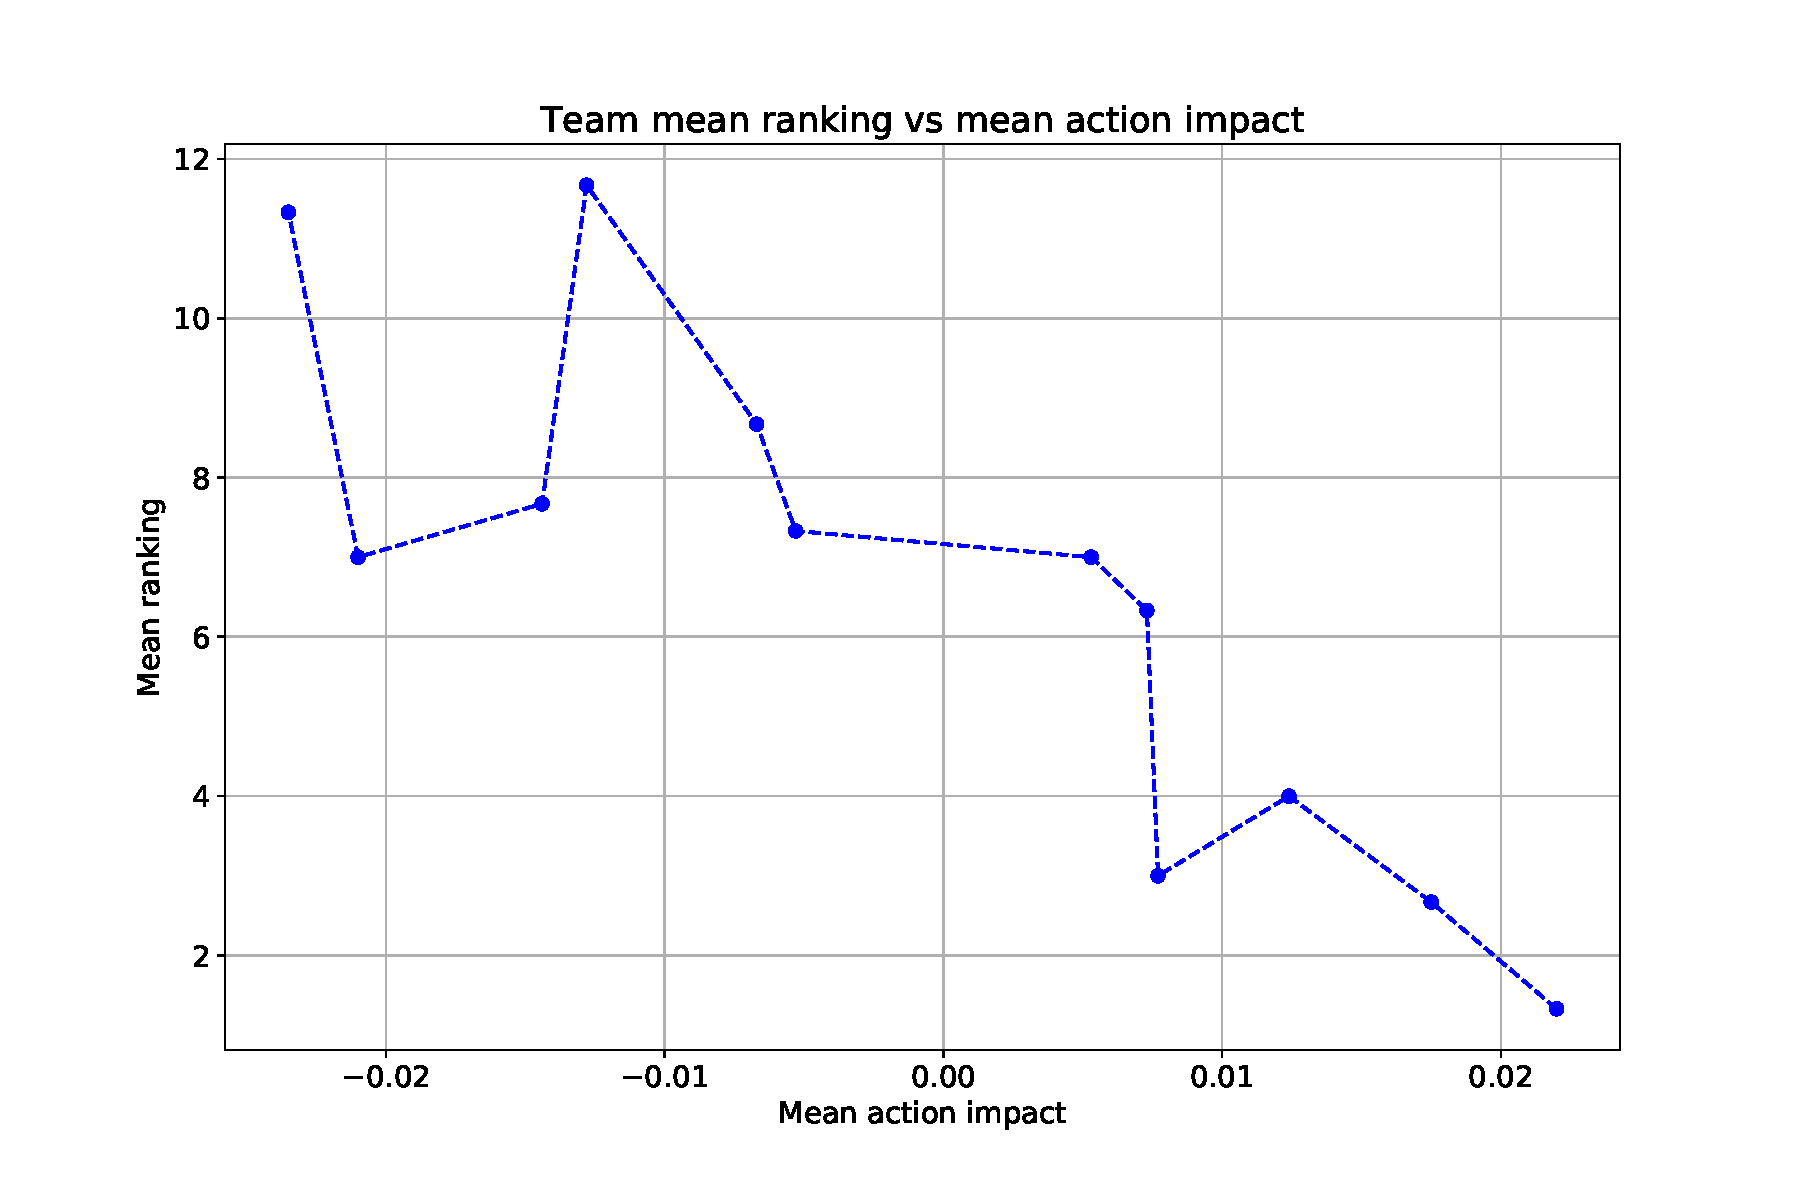
\includegraphics[scale=0.55]{img/team_ranking.pdf}
		\caption{Team mean ranking plotted against mean action impact for Canada West participating teams, see Table \ref{tab:team-impact} for values shown in this graph.}
		\label{fig:team-impact}
	\end{figure}
	
	%   BACK MATTER  %%%%%%%%%%%%%%%%%%%%%%%%%%%%%%%%%%%%%%%%%%%%%%%%%%%%%%%%%%%%%%
	%
	%   References and appendices. Appendices come after the bibliography and
	%   should be in the order that they are referred to in the text.
	%
	%   If you include figures, etc. in an appendix, be sure to use
	%
	%       \caption[]{...}
	%
	%   to make sure they are not listed in the List of Figures.
	%
	
	\backmatter%
	\addtoToC{Bibliography}
	\bibliographystyle{plain}
	\bibliography{msc_report}
	
	\begin{appendices} % optional
		\chapter{Code}
	\end{appendices}
\end{document}
